\documentclass[a4paper,10pt]{article}
\usepackage[utf8]{inputenc}
\usepackage[hyphens]{url}
\usepackage{graphicx}
%opening
\title{Machine Learning Engineer Nanodegree\\Captone Proposal}
\author{Sebastian Schmitz}

\begin{document}

\maketitle
\clearpage

\section{Domain background}
% (approx. 1-2 paragraphs)
% 
% In this section, provide brief details on the background information of the domain from which the project is proposed. Historical information relevant to the project should be included. It should be clear how or why a problem in the domain can or should be solved. Related academic research should be appropriately cited in this section, including why that research is relevant. Additionally, a discussion of your personal motivation for investigating a particular problem in the domain is encouraged but not required.
% 
Ever since Tesauro's backgammon agent TD-Gammon \cite{Tesauro:1995:TDL:203330.203343} proved that computer programs can perform as good as humans in certain games, machine learning algorithms have been applied in numerous games.
This lead to advances on both sides: The machine learning community could refine and improve their algorithms and the gaming communities learned new ways to play.

TD-Gammon used openings that had wrongfully been regarded as inferior by the leading players in the world. 
After a few tournaments where players tested the more conservative moves chosen by TD-Gammon, they became the near-universal choice, because they are - in fact - superior\cite{TDGammonArticle}.

One of the pinnacles of this development was reached when the AlphaGo computer program defeated the European Go champion Fan Hui on a full 19x19 board\cite{AlphaGoBeatsFanHui}. Until then, Go\cite{GoWiki} had been regarded as too complex to be mastered by an artificial intelligence.

Fueled by this development artificial intelligence programs trained through various forms of reinforcement learning\cite{ReinforcementLearningWiki} have learned to fly helicopters \cite{NIPS2006_3151}, play soccer \cite{Merke2002} and optimize stock trade execution \cite{Nevmyvaka:2006:RLO:1143844.1143929}.

Inspired by the ability of letting an agent learn how to thrive in an environment without being told what to do, I developed a reinforcement learning agent which solved a version of the game Rush Hour\footnote{\url{https://en.wikipedia.org/wiki/Rush_Hour_(board_game)}}.
The game consists of a 2d board with wooden pieces on it. The goal is to bring one of the pieces into a special position only by moving the blocks left, right, up or down.
My approach was able to find a solution that was a lot shorter than the solution that came with the game.

I now want to build upon this and move from a discrete problem to a continuous one.


\section{Problem statement}
% (approx. 1 paragraph)
% 
% In this section, clearly describe the problem that is to be solved. The problem described should be well defined and should have at least one relevant potential solution. Additionally, describe the problem thoroughly such that it is clear that the problem is quantifiable (the problem can be expressed in mathematical or logical terms) , measurable (the problem can be measured by some metric and clearly observed), and replicable (the problem can be reproduced and occurs more than once).
As an exercise to learn C++ and take a first peak into game programming, I programmed a 2d space game at the beginning of my studies in 2010, see figure \ref{fig:game}.
The goal of the game is to reach a score as high as possible by surviving and shooting down asteroids.
These asteroids spawn at random positions on the top of the screen and can either hit the player's ship making him lose a life or hit the off-screen space station which the player is supposed to protect. The space station gets repaired over time, but the player will lose if its health drops below $0$.
It might therefore be wise to crash the ship into an asteroid if it cannot be stopped otherwise and the space station is at low health.
In other situations it could be beneficial to let the asteroids hit the space station, since its health bar is still full.
Additionally, the amount of shots the player can fire at a time is limited, so it's not feasable to just fire at will.

The task of this project is therefore to let a machine learning algorithm figure out how to achieve the highest score.
In order not to bias the learning agent, no human-devised strategies will be programmed into the approach.
This will lead to an algorithm that potentially uses methods a human would not have thought of and that can cope with any of the random situations, the game throws at it.

\begin{figure}
 \centering
 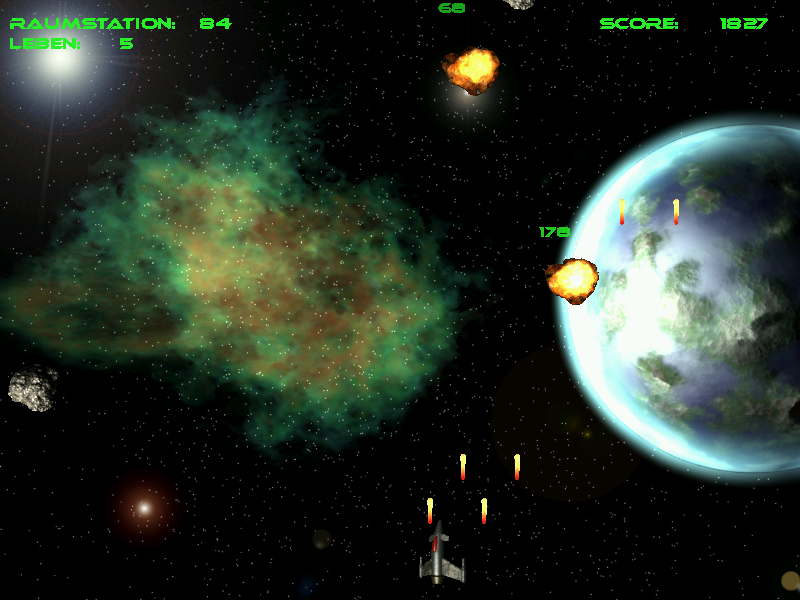
\includegraphics[width=\linewidth]{game2.png}
 \label{fig:game}
 \caption{2d space game}
\end{figure}

\section{Dataset and Inputs}
% (approx. 2-3 paragraphs)
% 
% In this section, the dataset(s) and/or input(s) being considered for the project should be thoroughly described, such as how they relate to the problem and why they should be used. Information such as how the dataset or input is (was) obtained, and the characteristics of the dataset or input, should be included with relevant references and citations as necessary It should be clear how the dataset(s) or input(s) will be used in the project and whether their use is appropriate given the context of the problem.
Since this is a simulation on a custom game there is no dataset to use.
The inputs the algorithm can make use of are the following:
\begin{itemize}
 \item Lifes left: Every time the space ship gets hit by an asteroid, the player will lose a life and eventually the entire game if no lives are left.
 \item Space station health: Every time an asteroid is allowed to cross the screen, the space station will lose a set amount of health and regenerate it at a fixed rate until it's back at 100 again. If the space station health drops below $0$, the player will lose the game.
 \item Asteroids: Set of x- and y-coordinates describing the positions of the asteroids
 \item Ship position: The ship can move left and right on the lower corner of the screen
 \item Shots left: Only a certain amount of shots can be fired at a time.
 \item Shot positions: Set of x- and y-coordinates of the shots the player has already fired.
\end{itemize}

\section{Solution statement}
% (approx. 1 paragraph)
% 
In the MLND lectures we learned about three fields of machine learning: Supervised learning, unsupervised learning and reinforcement learning.
The proposed problem does not include large datasets that we can mine for information which we would need to apply (un)supervised learning methods. 
It is rather an environment in which an algorithm has to learn over time, adapt to so far unseen  situations and generalize the experiences made in order to be able to handle as many problems that can arise within this environment as possible.

The solution will therefore leverage the strength of algorithms coming from the field of reinforcement learning:
The system will start with no knowledge about the problem whatsoever, but it will perceive the state of the environment and will be able to derive a set of actions from this state.
At first, the actions taken will be randomly chosen: 
The environment transitions into another state and the agent will immediately receive feedback on whether the choice of action was good or not.
From these feedbacks the algorithm will over time create a graph modelling the environment:
The nodes will be the states, the edges and their weights will be the actions.
Since the goal is to learn how to behave, the level of randomness when choosing actions will be decreased by a small amount with every run.
This leads to a transition in the behavior: In the beginning, the agent will explore the environment and after some time start exploiting its knowledge to ensure that the best solution was found.

The result will be an agent that has explored a big portion of the state space and can play the game reasonably well, ideally better than a human player.
% In this section, clearly describe a solution to the problem. The solution should be applicable to the project domain and appropriate for the dataset(s) or input(s) given. Additionally, describe the solution thoroughly such that it is clear that the solution is quantifiable (the solution can be expressed in mathematical or logical terms) , measurable (the solution can be measured by some metric and clearly observed), and replicable (the solution can be reproduced and occurs more than once).


\section{Benchmark Model}
% (approximately 1-2 paragraphs)
% 
% In this section, provide the details for a benchmark model or result that relates to the domain, problem statement, and intended solution. Ideally, the benchmark model or result contextualizes existing methods or known information in the domain and problem given, which could then be objectively compared to the solution. Describe how the benchmark model or result is measurable (can be measured by some metric and clearly observed) with thorough detail.

Since the agent will train on a custom game, the choice of benchmark models and solutions to compare the performance to is sparse:



% Since the agent will train on a custom game, there does not exist a benchmark yet which its performance can be compared to.
% However, it is possible to objectively measure the effectiveness of the agent's actions and how it improves  over time:
% The overall score of the game is what defines the quality of the actions taken either by an artificial player as well as by a human.
% Hence, if the agent is able to perform at a level on par with a human player, I will consider my goal reached.

\section{Evalution Metrics}
% (approx. 1-2 paragraphs)
% 
% In this section, propose at least one evaluation metric that can be used to quantify the performance of both the benchmark model and the solution model. The evaluation metric(s) you propose should be appropriate given the context of the data, the problem statement, and the intended solution. Describe how the evaluation metric(s) are derived and provide an example of their mathematical representations (if applicable). Complex evaluation metrics should be clearly defined and quantifiable (can be expressed in mathematical or logical terms).
\section{Project Design}
% (approx. 1 page)
% 
% In this final section, summarize a theoretical workflow for approaching a solution given the problem. Provide thorough discussion for what strategies you may consider employing, what analysis of the data might be required before being used, or which algorithms will be considered for your implementation. The workflow and discussion that you provide should align with the qualities of the previous sections. Additionally, you are encouraged to include small visualizations, pseudocode, or diagrams to aid in describing the project design, but it is not required. The discussion should clearly outline your intended workflow of the capstone project.




\bibliographystyle{plain}
\bibliography{bib}
\end{document}
